\section{Background}

We present some of the background material in this section that would prepare
us for the latter part of the article. 
In particular, we present an overview of metadata-based recovery and file carving. 
Then, we present the NIST CFTT expectations for such recovery tools.  


\subsection{Metadata-based deleted file recovery}
This recovery mechanism relies on the residual metadata of the deleted files, 
which are still present in the file system. Note that in a typical file system 
a file has some metadata in addition to the actual file content. However,
different file systems
manage the metadata in different ways.
In Section \ref{subsubsec:fat-overview} and Section \ref{subsubsec:ntfs-overview}, 
we present an overview of FAT and NTFS file systems, respectively, which is often
simplified to aid readability. 
Then, in Section \ref{subsubsec:meta-recovery}, we discuss how metadata can help in 
recovery of a deleted file.

\subsubsection{FAT File System} \label{subsubsec:fat-overview}

For a file, FAT file system maintains an important piece of metadata, 
which is known as \emph{directory entry} and is of 32 bytes, containing three 
key elements: (i) name of the file (say bar.txt), (ii) size of the file, and 
(iii) index of the starting cluster that hosts the file content. 
The file system maintains the index of the other clusters of the file (bar.txt) 
via a global table known as the FAT table. For each cluster, 
there is an entry in the FAT table, which holds the status 
(allocated vs. unallocated) of the cluster, and if allocated, 
it also tells us what the next cluster is. In particular, if $x^{th}$ entry is $0$, 
we infer that the cluster is unallocated. Otherwise, if $x^{th}$ entry is $y$, then 
that means the next cluster after cluster $x$ (as part of the same file) is $y$.
When $x^{th}$ entry holds a special value called EOF, we infer that cluster $x$ is
the last cluster of the file.

For instance, Figure~\ref{fig:fat1} illustrates the directory entry and data clusters of 
a file bar.txt. The FAT table is also shown. We can infer from the FAT table that the file's
(bar.txt) content is stored in contiguous clusters, from cluster 200 to cluster 204.


\begin{figure}[h]
     \centering
     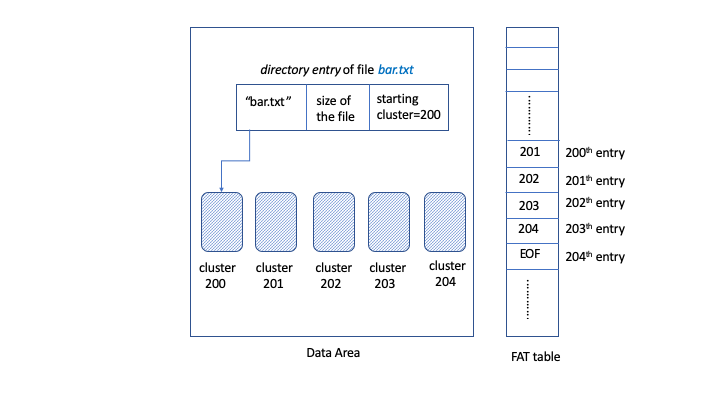
\includegraphics[width=\linewidth]{fig/fat1.png}
     \caption{The actual data part and metadata of file bar.txt in a FAT file system. The \emph{directory entry} of this file and the actual file content clusters (shaded) are shown. The FAT table is also shown.}
     \label{fig:fat1}
 \end{figure}

When a file is deleted in FAT system, most of the actual content and metadata might 
remain intact in many cases. 
Figure~\ref{fig:fat2} illustrates the status of the file system after the file bar.txt is deleted.
All fields of the directory entry remain unchanged except the first character of the file name 
is replaced with an underscore (`\_') to flag the \emph{deleted} status. The main change happens in the FAT table where all entries
that were associated with bar.txt are \emph{zeroed}. However, the clusters (holding the file content) 
remain intact until some other file (partially or fully) \emph{overwrites} them. 

  
\begin{figure}[h]
    \centering
    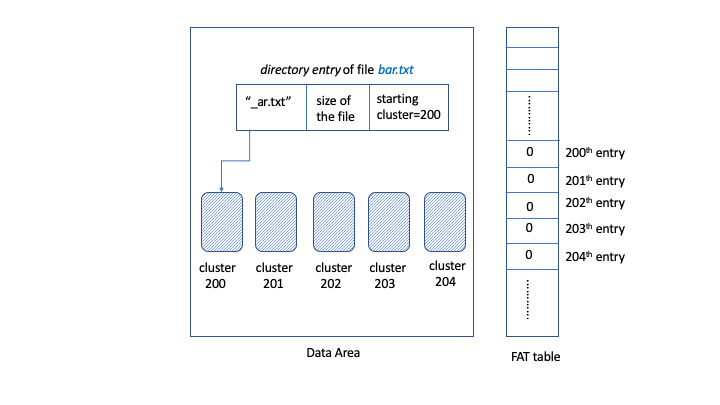
\includegraphics[width=\linewidth]{fig/fat2.png}
    \caption{The actual data part and metadata of bar.txt after the file is deleted whereas its entries in the FAT table (i.e., entry $200$ to entry $204$) are zeroed.}
    \label{fig:fat2}
\end{figure}

So far, we have considered a file whose actual content is stored in contiguous clusters. 
It is also possible that a file's content is not stored in contiguous clusters, and such a file is 
called a \emph{fragmented} file. Figure~\ref{fig:fat3} illustrates an example where file bar.txt is fragmented.

 \begin{figure}[h]
     \centering
     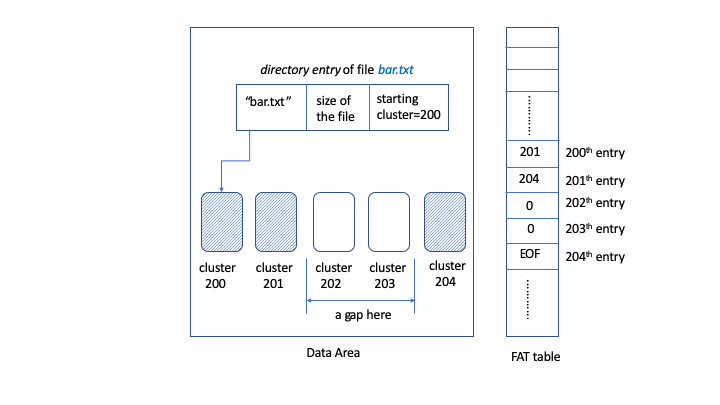
\includegraphics[width=\linewidth]{fig/fat3.png}
     \caption{The actual content and metadata of bar.txt is shown. Per the FAT table the file has two fragments (cluster 200-201 and cluster 204).}
     \label{fig:fat3}
 \end{figure}



\subsubsection{NTFS File System} \label{subsubsec:ntfs-overview}

NTFS file system does not maintain a global table (like the FAT table) 
that holds the status for each cluster. Instead NTFS maintains a global table called 
MFT (Master File Table) that
holds information for each file in the system. In particular, each file $f$ has an 
entry in MFT, which holds information about file $f$, and the size of this entry is 1024 bytes.  
If file $f$ is a small file, then the whole file content as well as the metadata will be stored
inside $f$'s MFT entry; 
otherwise, $f$'s content is \emph{non-resident} and is stored in other clusters. 
Figure~\ref{fig:ntfs} illustrates an example where the file bar.txt's content is non-resident, 
and it has two fragments. When a file $f$ is deleted in NTFS, 
the corresponding entry in MFT is flagged as deleted and the corresponding clusters 
(if any) are flagged as deleted, but the metadata and file content remain intact otherwise.
Note that NTFS file system does not have specific zones for data area in contrast of 
FAT having specific area for data and specific area for the FAT table.


 \begin{figure}[h]
     \centering
     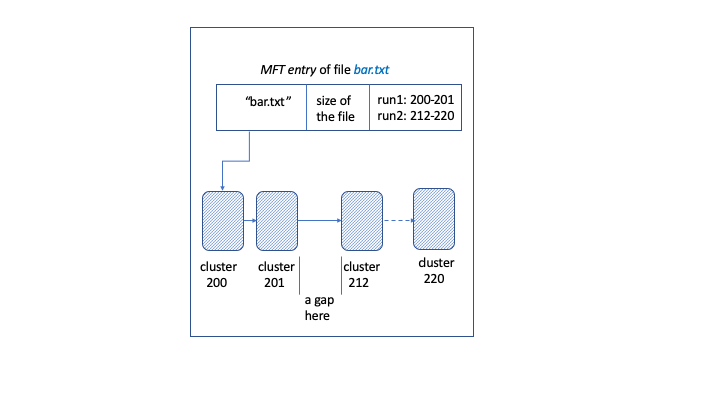
\includegraphics[width=\linewidth]{fig/ntfs.png}
     \caption{To illustrate NTFS file system, the MFT entry of foo.txt and the actual content carrying clusters are shown. 
 This file has two fragments (cluster 100-101 and cluster 200-298).}
     \label{fig:ntfs}
 \end{figure}
 

\subsubsection{Recovering deleted files}\label{subsubsec:meta-recovery}

From the previous discussion we note that in many situations the metadata
(e.g., directory entry in FAT or MFT entry in NTFS) of the deleted file remains
unchanged and can be used for identifying and recovering the deleted file.
As an example, the directory entry of bar.txt in Figure~\ref{fig:fat2} tells us
that the file's content starts from cluster $200$, 
and using the \emph{size} field value (e.g., $5$) we can infer that the file's content
is hosted in the cluster chain from cluster $200$ to cluster $204$, assuming that there is no
fragmentation. We can recover the file via reading the raw content of these $5$ clusters, e.g.,
by using dd command in Linux.  

We encounter one critical challenge while recovering a fragmented file in FAT because \emph{directory entry}
of a file does not contain any information about the fragments. However, we do not face this challenge 
in file recovering in NTFS because MFT entry (as shown in Figure~\ref{fig:ntfs}) does contain the start and end cluster index for each run (i.e., fragment). 

\subsection{File Carving}\label{subsec:file-carving}

File carving does not rely on the file system metadata, and hence is independent of the type of the 
file system (e.g. FAT vs. NTFS). In file carving, we assume that the target file has 
a known header and footer signature (i.e., a sequence of special bytes). As an example, 
jpg files have such header and footer signature. The file carving process basically
scans the whole storage space (i.e. the target storage device where we plan to recover deleted files from) 
byte by byte and identifies each match of header and footer signature. 
Then, the content between any header and any footer is potentially a recovered file. 
Depending on the strong vs weak match policy, there could be \emph{false positives} 
(i.e., bogus files being retrieved) 
and \emph{false negatives} (i.e., files missed to be retrieved). 

\subsection{NIST Guidelines}
\subsubsection{For Metadata-Based DFR}
\begin{paraphrase}
 The NIST guidelines~\cite{meta:dfr:standards} list four \emph{core features} upon which metadata-based DFR tools are to be judged.
Following is the text of each core feature as well as our interpretation of each in the context of this work:

 \paragraph{DFR-CR-01} ``The tool shall identify all deleted File System-Object entries accessible in residual metadata''~\cite{meta:dfr:standards}.
 We consider a tool passing this standard if it identifies to the user each file system metadata entry that is marked as deleted.
 \paragraph{DFR-CR-02} ``The tool shall construct a Recovered Object for each deleted File System-Object entry accessible in residual metadata''~\cite{meta:dfr:standards}.
 We consider a tool passing this standard as long as it outputs a file for each deleted file, even if the output file is empty.
 \paragraph{DFR-CR-03} ``Each Recovered Object shall include all non-allocated data blocks identified in a residual metadata entry''~\cite{meta:dfr:standards}.
 For FAT file systems, we consider a tool passing this standard if it recovers at least the first contiguous segment of unallocated sectors starting 
from the first sector originally allocated to the deleted file. For NTFS file systems, the tool must recover all unallocated sectors originally allocated to the deleted file.
 \paragraph{DFR-CR-04} ``Each Recovered Object shall consist only of data blocks from the Deleted Block Pool''~\cite{meta:dfr:standards}.
 We consider a tool passing this standard if the recovered file consists only of data from the original deleted file, or null data to represent omitted portions.


\end{paraphrase}

\subsubsection{For File Carving} \label{sec:carving_features}

\begin{paraphrase}
 The NIST guidelines~\cite{carving_standards} list five \emph{core features} upon which file carving DFR tools are to be judged.
Following is the text of each core feature as well as our interpretation of each in the context of this work:
\end{paraphrase}

 \paragraph{FC-CR-01} ``The tool shall return one carved file for each supported file header signature from a source file that is present in the search arena''.~\cite{carving_standards}
 
 Each file from the original disk will begin with a header signature specific to its file format. We consider a tool as passing this guideline if it carves a file starting at each of those header signatures.
 In other words, tools that perform well on this core feature have a high ``hit rate.''
 
 \paragraph{FC-CR-02} ``A carved file shall only contain data blocks from the search arena''.~\cite{carving_standards}
 
 In other words, the tool should only work within the drive or partition it is given, and should not try to carve from out-of-bounds.
 
 \paragraph{FC-CR-03} ``All data blocks in a carved file shall originate in a single source file''.~\cite{carving_standards}
 
We consider a tool as passing if each recovered file only contains data from one file on the original disk.
 
 \paragraph{FC-CR-04} ``The file type of a carved file shall match the file type of its contents''.~\cite{carving_standards}
 
 We interpret this to mean that the file extension given to a recovered file must accurately describe the format of the file data. We exclude false positives from this evaluation because their data is highly unlikely to be of any file format. So, we only consider files which were carved starting from a valid header signature.
 
 \paragraph{FC-CR-05} ``The tool shall return carved files in a state that conforms to a valid file of the carved file type''.~\cite{carving_standards}
 
 We consider a tool as passing if each recovered file can be parsed without error by some application software.
 We use the ImageMagick tool suite to evaluate this.
